\section{Methods \& Materials}
\label{sec:Methods-Materials}

\subsection{Tools}

To construct our simulation environment, and due to the goal of creating a simple simulation, prioritizing understanding of the models over their precision, rather simple tools were used, which do not provide specific tools for road network and vehicle-related simulation. The Mesa \footnote{\url{https://mesa.readthedocs.io/en/latest/index.html}} Agent-based simulation Python library was used to construct the main simulation logic. Mesa focuses on being a straightforward tool that enables beginners to create agent-based simulations with a discrete time step, revolving heavily around a structure composed of agent objects that implement a step function, in which all decision-making is executed. Mesa provides some different simplistic ways for visualization and allows for direct integration for visualization of graphs built using NetworkX \footnote{\url{https://networkx.org/}}, another simple tool for graph networks management and related operations, including algorithm implementations for the most common graph-related problems, such as shortest path. Another important tool for the realization of the project was Matplotlib \footnote{\url{https://matplotlib.org/}}, a Python library that possibilities the construction of elegant graph plots, which has seamless integration with the visualization mechanisms of Mesa as well.

\subsection{Simulation Environment Definition}

\textbf{Entities:}
\begin{itemize}
    \item Vehicles
\end{itemize}

\textbf{Resources:}
\begin{itemize}
    \item Route/Road Space
\end{itemize}

\textbf{Exogenous Variables:}
\begin{itemize}
    \item \textbf{Uncontrollable:}
    \begin{itemize}
        \item \textbf{Traffic Network Configuration:} the node and edges of the graph network;
        \item \textbf{Vehicle Arrival Rate:} the amount of vehicles arriving at the network in the start node per time step;
        \item \textbf{GPS Usage Ratio:} probability of using the Intelligent GPS instead of base policy (explained further ahead)
    \end{itemize}
    \item \textbf{Controllable:}
    \begin{itemize}
        \item Information Percolation Method - Vehicle Route Decision Strategy 
    \end{itemize}
\end{itemize}

\textbf{Endogenous Variables:}
\begin{itemize}
    \item \textbf{Average Travel Efficiency at 200 (ATE200):} the ratio between the shortest time necessary for the completion of a path without traffic with the average travel time (when the 200th vehicle finishes the path) - performance metric chosen due to its capability of informing on the throughput of a network regardless of its structure and of the goal path's length;
    \item \textbf{Average Travel Time at 200:} average time taken by a vehicle to cover the (when the 200th vehicle finishes the path) - performance metric chosen for its simplicity in portraying the throughput of the network;
    \item \textbf{Max Volume to Capacity Ratio at 200:} illustrates the maximum congestion of any route in the network (when the 200th vehicle finishes the path) - performance metric chosen for its simplicity in defining the unbalance between roads;
    \item \textbf{Steps until 200:} number of simulation steps (mins) until 200 vehicles complete the path - performance metric chosen due to clearly showing the difference between models for the same network in throughput, as it is not averaged and reflects the efficiency for a fixed number of vehicles; 
\end{itemize}

\textbf{Events:}
\begin{itemize}
    \item Vehicle entering the network
    \item Vehicle leaving the network
\end{itemize}

\textbf{Performance Indicator:} ATE200 $>$ 0.4

\textbf{Decision Criteria:}
\begin{itemize}
    \item If the CAV Model presents an improvement in ATE200 of more than 0.1 compared to the Descriptive Models, then the adoption of CAVs should be taken as a serious solution for traffic congestion problems
    \item If a Model fulfils the performance indicator, its usage is deemed justified by this experiment
\end{itemize}

\subsection{Road Network Modelling}

In order to represent the road network in the simulation, it was decided that a graph representation was the most suitable. In this graph representation, the nodes would correspond to the intersections of the edges, while the edges represent the roads themselves. 

The graph is a \textbf{directed graph}. For each road network, a start node and an end node are always defined. The edges' weights correspond to the estimated cost of their traversal, varying for each operation policy. A few networks were modelled, representing slightly different levels of complexity. They ought to represent connections of highways and large roads between an origin and a destination. The main ones used in the tests are represented in Figures \ref{fig:medium-road-network} and \ref{fig:large-road-network}.

\begin{figure}
    \centering
    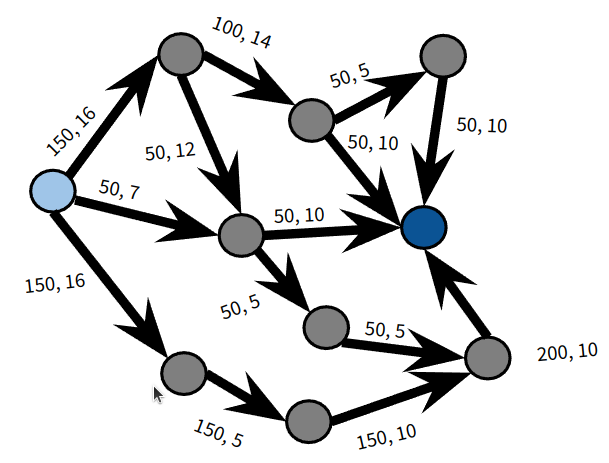
\includegraphics[width=0.4\textwidth]{img/large.png}
    \caption{Large Road Network}
    \label{fig:large-road-network}
\end{figure}

\begin{figure}
    \centering
    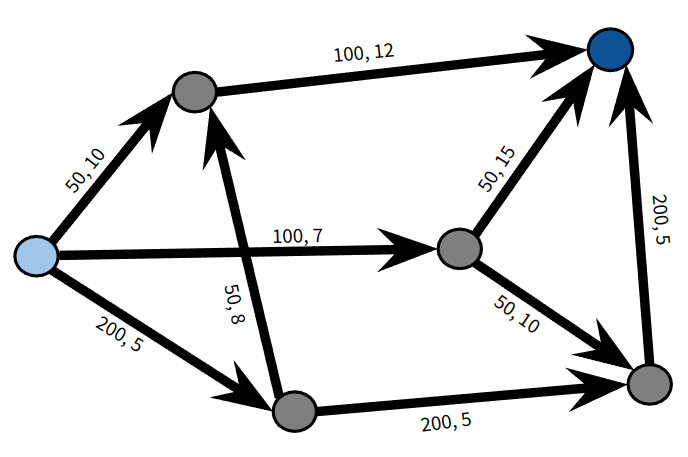
\includegraphics[width=0.4\textwidth]{img/medium.png}
    \caption{Medium Road Network}
    \label{fig:medium-road-network}
\end{figure}

\subsection{Route Choice Models}

Our simulation environment naturally defines multiple models for the representation of the road network, such as the vehicle flow model, which defines the flow of the vehicles on the network dependent on the route's characteristics and its current state regarding the vehicles that occupy it. Even so, there is only one model which is the target of this study, the route decision model: which defines the strategy followed by the agents (vehicles) for the decision between two or more different routes from their current point to their objective. This model naturally corresponds to the \textbf{operation policy} of our simulation. Taking this into account, three different models evaluated were:

\begin{itemize}
    \item \textbf{Base model:} Descriptive model based on the behaviour a vehicle would depict if the driver knew the shortest route but was oblivious to the current state of the road network in terms of volume distribution. It emulates a driver following a map or a simple GPS. Programmatically, it is emulated by having the vehicles always follow the shortest path between their current point and goal point, having this path been calculated using the free-flow time of the roads as the weights for the edges.
    \item \textbf{Intelligent GPS model:} Descriptive model attempting to represent the behaviour of a vehicle whose driver uses an application such as Google Maps, which calculates the best route taking into account the congestion of the roads in the road network, with a natural certain delay. This behaviour is coded by having the vehicles always follow the shortest path between their current point and goal point, having this path been calculated using the BPR function on the roads at a few steps prior, representing the delay in these applications.
    \item \textbf{Connected Autonomous Vehicles model:} Speculative model which describes the behaviour of the vehicles in a hypothetical scenario where they have information in real-time of the number of vehicles in each route they could opt upon and could therefore predict with very high accuracy the route with lowest travel time. This behaviour is coded by having the vehicles always follow the shortest path between their current point and goal point, having this path been calculated using the BPR function on the roads at the moment of choice, representing the instant knowledge provided by a network of autonomous vehicles, constantly in communication.
\end{itemize}

\subsection{Network Flow Modelling}

Simulating the movement of a vehicle in a road network is fundamental for the simulation task at hand. Not only that, but the travel time of the vehicle on a certain road or route should be dependent on the road's characteristics, most importantly its state at a given point in time regarding the congestion, as it is a direct function of the choices made by the drivers and impacts the network's throughput and average travel time. In order to model the movement of the vehicles and its conditioning by the state of the route at a given point in time, we chose to use the BPR (Bureau of Public Roads) function. It is a function that defines the travel time of a given vehicle through a route in function of the capacity of the route and its current volume, as well as the free-flow travel time. 

\begin{equation} \label{eq:bpr}
    T_a  = T_f \times (1 + \alpha \times (\frac{V}{C})^\beta)
\end{equation}

where:

\begin{itemize}
    \item $T_a$ is the travel time for a vehicle entering the road
    \item $T_f$ is the travel time for that road under free flow conditions (no traffic)
    \item $V$ is the current volume of the road (number of vehicles)
    \item $C$ is the capacity of the road (number of vehicles)
    \item $\alpha$ and $\beta$ are two configurable parameters. The  $\alpha$ parameter is the ratio of travel time per unit distance and $\beta$ determines how fast the curve increases from the free-flow travel time \cite{anwar2011newly}
\end{itemize}

For our experiments, we assigned the most typical values for the two constants \cite{gore2023modified}, having defined $\alpha = 0.15$ and $\beta = 4.0$.

At each time step, the agents on the simulation (the vehicles) will increment a counter denoting the progress on a given road. The vehicle will only exit the road when this counter reaches a value calculated at the point the agent made the choice to enter it. This value is exactly the value given by the BPR function, using the $C$ and $V$ values of the road in which the vehicle is entering at the moment he is entering.

\subsection{Verification}

The model was verified through extensive unit testing of the used classes with the \textit{Pytest} framework. It successfully passed all the tests it was put through, resulting in the verification of its operation inside the context of the simulation model we aimed to build and its assumptions.
